% (C) 2013 - Université de Strasbourg
% * Guillaume Dollé <guillaume.dolle@math.unistra.fr>
% * Christophe Prud'homme <christophe.prudhomme@feelpp.org>
% Tutorial documentation - mymesh
%

\section{Diffusion advection reaction problem}
\label{sec:tuto-myadvection}

The diffusion advection reaction equation is a classical partial differential
equation which can be found in many processes for example in chemistry or
biology. This can be described by an equation containing a diffusion, an
advection and a reaction term as follows,
%
\begin{equation}
  \left\{
    \begin{array}{rcll}
      -\epsilon\Delta  u + \bbeta \cdot \nabla  u + \mu u & = & f & \text{on}\; \Omega \;, \\
      u  & = & 0 & \text{on}\; \partial\Omega \;, \\
    \end{array}
  \right.
  \label{eq:tuto-adv}
\end{equation}
%
We use here homogeneous Dirichlet boundary conditions.

\subsubsection{Variationnal formulation}

To establish the variationnal formulation, as always we mutiply the first equation by a
test function $v\in H_0^1(\Omega)$ such that,
\[
    H_0^1(\Omega) = \{ v\in H^1(\Omega),\; v=0 \; \text{on} \; \partial\Omega \} \;.
\]
Then we integrate on the domain $\Omega$,
%
\begin{equation}
- \int_\Omega \epsilon \Delta u\ v
+ \int_\Omega \bbeta \cdot \nabla u\ v
+ \int_\Omega \mu\ u\ v
= \int_\Omega f\ v \;.
\end{equation}
%
We establish the variationnal formulation from the previous equation and using
the Green formula, find $u \in \in H_0^1(\Omega)$
%
\begin{equation}
  \int_\Omega \epsilon \nabla u \cdot \nabla v
  - \underbrace{\int_{\partial\Omega} \epsilon (\nabla u \cdot \mathbf n)\ v}_{=0}
  + \int_\Omega (\bbeta \cdot \nabla u)\ v
  + \int_\Omega \mu\ u\ v
  = \int_\Omega f v \; \quad \forall v \in \in H_0^1(\Omega),
  \label{eq:tuto-adv-varform}
\end{equation}
%
where $\mathbf n$ is a unit outward normal vector. We can rewrite the problem,
find $u \in \in H_0^1(\Omega)$
%
\begin{equation}
    a(u,v) = l(v) \quad \forall v \in \in H_0^1(\Omega),
\label{eq:tuto-adv-bilform}
\end{equation}
%
where $a$ is a bilinear form, continuous, coercive and $l$ is a linear form.

\subsubsection{Application}

We choose for our example $\mu = 1$, $\epsilon = 1$, $f=1$, and
$\bbeta=(1,1)^T$.

%
\vspace{2mm}
\lstinputlisting[linerange=marker_main-endmarker_main, caption={\lstinline{doc/manual/tutorial/myadvection.cpp}}]{tutorial/myadvection.cpp}
\vspace{2mm}
%
Again the implementation is close to the mathematical formulation.  Here again,
we create the mesh for an unit square geometry. Then we define the function
space $X_h$ we choose as order 1 Lagrange basis function using
\lstinline!Pch<Order>()!.  Note that here, the function space is the same for
"trial" and "test" functions.  We declare the left and the right hand side
integrals expressions for the equation (\ref{eq:tuto-adv-varform}). Finally we
add the Dirichlet boundary condition and we use the default solver to solve
(\ref{eq:tuto-adv-bilform}).  We export the solution $u$ for post processing.



\begin{figure}[htbp]
  \centering
  \subfigure[$\epsilon=1$]{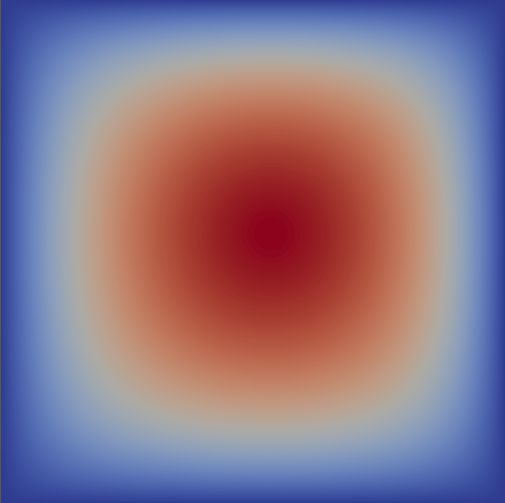
\includegraphics[width=.3\linewidth]{pngs/myadvection/sol-dar-1.png}}
  \subfigure[$\epsilon=0.01$]{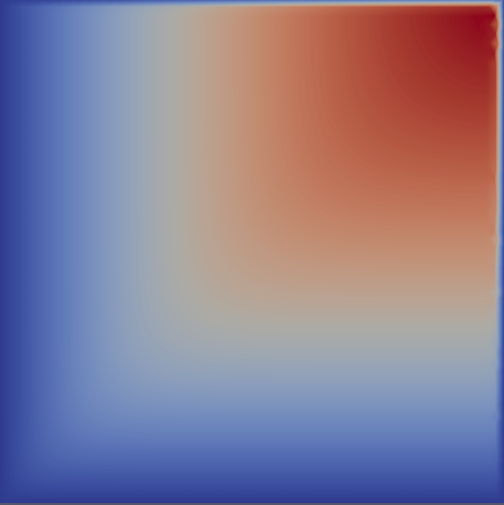
\includegraphics[width=.3\linewidth]{pngs/myadvection/sol-dar-2.png}}
  \subfigure[$\epsilon=0.0001$]{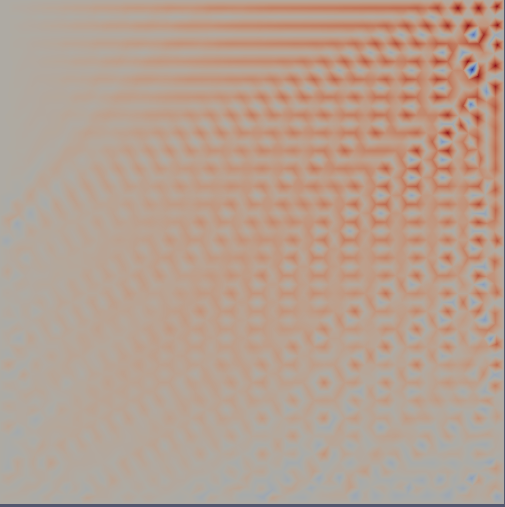
\includegraphics[width=.3\linewidth]{pngs/myadvection/sol-dar-3.png}}
  \caption{Various solutions of problem~\eqref{eq:tuto-adv-bilform}  for $\epsilon=1,0.01,0.0001$. Notice how
  the solution gets unstable for $\epsilon=0.0001$, this is classical and
  requires stabilisation methods to handle this issue.}
  \label{fig:tut:1}
\end{figure}

%%% Local Variables:
%%% coding: utf-8
%%% mode: latex
%%% TeX-PDF-mode: t
%%% TeX-parse-self: t
%%% x-symbol-8bits: nil
%%% TeX-auto-regexp-list: TeX-auto-full-regexp-list
%%% TeX-master: "../feelpp-manual"
%%% ispell-local-dictionary: "american"
%%% End:

